% ******************************* Thesis Appendix A ****************************
\chapter{TRECVID MED 2013 Results} 

\ifpdf
\graphicspath{{Appendix1/Figs/Raster/}{Appendix1/Figs/PDF/}{Appendix1/Figs/}}
\else
\graphicspath{{Appendix1/Figs/Vector/}{Appendix1/Figs/}}
\fi

In this appendix, we briefly introduce our Multimedia Event Detection system for TRECVID MED 2013. We use both audio and visual features with Bag-of-Words and Fisher Vector Representation. Our MED framework consists of following steps: preprocessing, feature extraction, feature representation and event classification.

\textbf{Preprocessing.} At first, all videos are normalized to around 320x240. We fix the width dimension to 320 and change the height so that the aspect ratios are kept. The audio channels are removed from resized videos to save disk space. After that, we extract one representative keyframe from resized videos at every 2 seconds and audio feature from the original videos. 

\textbf{Feature Extraction.} We use feature from different modalities to model multimedia events: still image features, motion features and audio features. We use the standard SIFT with Hessian Laplace detector for extracting still image feature. For motion feature, we use Dense Trajectories with MBH descriptor. We use the MFCC for extracting audio feature. 

\textbf{Feature Representation.} Bag-of-Words representation is a simple way to encode local features. It is the frequency histogram of local descriptors that are assigned to the nearest clusters. In the implementation, we randomly select 1,000,000 local descriptors to train the codebook with 4,000 codewords. The soft assignment technique is also employed to reduce the quantization errors. For Fisher vector, we use the codebook size of 256 clusters which are generated using the Gaussian Mixture Model (GMM). We further improve the expressiveness of Fisher vector by applying PCA for reducing feature dimension, i.e 80-d for SIFT and 128-d for MBH. 

\textbf{Event Classification.}
We use the popular Support Vector Machine (SVM) for classification. All the positive videos are considered as positive samples and the remaining videos are considered as negative samples (including near miss videos). We use the chi-square kernel for training bag-of-words histogram features and linear kernel for training features encoded by Fisher vector.

\textbf{Results and Conclusion.} We observed that Fisher vector representation is consistently better the traditional bag-of-words histogram representation. The motion features archived the highest performance in terms of single feature comparison, followed by image features and audio features. Furthermore, these features are highly complementary, so their combination achieved the best performance. We also observed a little performance gain when combining both Fisher vector and bag-of-words feature encoding. Based on these observations, we submitted the FullSys system based on the combination of audio or visual features. Our results (NII Team) on the 100Ex setting is shown in Fig. \ref{med2013_result}. Our rank is 4th out of 18 participants.

\begin{figure}
	\centering
	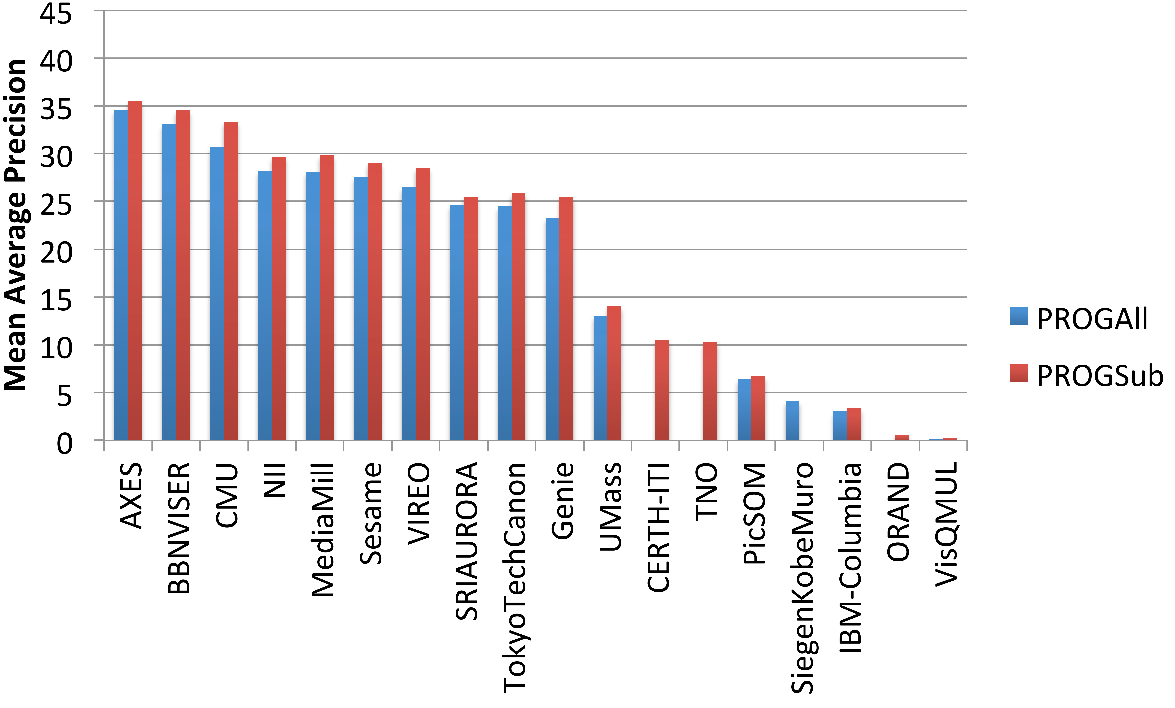
\includegraphics[width=1\textwidth]{results.pdf}
	\caption{Comparison of our MED 2013 system with others on the full evaluation set for the Pre-specified task. Results are sorted in the descending order of performance on the EK100 setting.}
	\label{med2013_result}
\end{figure} 